\documentclass[11pt,a4paper]{article}
\usepackage{graphicx}
\usepackage{subfigure}
\usepackage{amsmath}
\usepackage{makecell}
\usepackage[utf8]{inputenc}
\usepackage{listings} %放代码
\usepackage{xcolor} %代码着色宏包
\usepackage{xeCJK}
\usepackage{float}

\lstset{
	backgroundcolor=\color{white}, 
	%\tiny < \scriptsize < \footnotesize < \small < \normalsize
	basicstyle = \footnotesize,       
	breakatwhitespace = false,        
	breaklines = true,                 
	captionpos = b,                    
	commentstyle = \color{black}\bfseries,
	extendedchars = false,
	frame =shadowbox, 
	framerule=0.5pt,
	keepspaces=true,
	keywordstyle=\color{black}\bfseries, % keyword style
	language = C++,                     % the language of code
	otherkeywords={string}, 
	numbers=left, 
	numbersep=5pt,
	numberstyle=\tiny\color{black},
	rulecolor=\color{black},         
	showspaces=false,  
	showstringspaces=false, 
	showtabs=false,    
	stepnumber=1,         
	stringstyle=\color{mymauve},        % string literal style
	tabsize=4,          
	title=\lstname                      
}

%好像是数学的包
\usepackage{amsmath}
\usepackage{amssymb}
\usepackage{mathrsfs}
%页面布局包
\usepackage{geometry}
%画图包
\usepackage{tikz}
%画图背景包
\usetikzlibrary{backgrounds}

\geometry{left=3.0cm, right=3.0cm, top=3cm, bottom=3cm}

%自定义命令
\newcommand{\psiG}{\psi_{G}}
%在tikz中画一个顶点
%#1:node名称
%#2:位置
%#3:标签
\newcommand{\newVertex}[3]{\node[circle, draw=black, line width=1pt, scale=0.8] (#1) at #2{#3}}
%在tikz中画一条边
\newcommand{\newEdge}[2]{\draw [black,very thick](#1)--(#2)}
%在tikz中放一个标签
%#1:名称
%#2:位置
%#3:标签内容
\newcommand{\newLabel}[3]{\node[line width=1pt] (#1) at #2{#3}}
\newcommand{\keypoint}[1]{$\bullet$#1\par}
\newcommand{\jumpLine} {\hspace*{\fill} \par}




\title{Introduction to Computing Systems\\Homework 6}
\author{PB18111697 王章瀚}

\begin{document}
	\maketitle
	\section*{1.}
	\ \par
	\keypoint{The trap vector has 8 bits, which means up to 256 serveice routines can be specified.}
	\keypoint{We won't be sure about which address shall be filled into PC when returning, while the BRnzp can only set PC to a certain value. Instead, using the RET, PC will be set as the R7's value, which is variable.}
	\keypoint{1. The first is to access the vector table to get the service routine's address and load it into PC.}
	
	\section*{2.}
	\ \par
	The last thing you stored in it is the first thing you remove from it.\par
	One example is the behaviour of a coin holder. Another is in hardware-data entries move.\par
	The difference lies in whether remove the value after pop. In the first one, the value, which is the coins, will be removed, while in the second one, the value stays but the cursor moves.\par
	
	\section*{3.}
	\subsection*{a.}
	\begin{tabular}{|c|c|}
		\hline 
		push & Z \\ 
		\hline 
		push & Y \\ 
		\hline 
		pop & Y \\ 
		\hline 
		push & X \\ 
		\hline 
		pop & X \\ 
		\hline 
		push & W \\ 
		\hline 
		push & V \\ 
		\hline 
		pop & V \\ 
		\hline 
		push & U \\ 
		\hline 
		pop & U \\ 
		\hline 
		pop & W \\ 
		\hline 
		pop & Z \\ 
		\hline 
		push & T \\ 
		\hline 
		push & S \\ 
		\hline 
		pop & S \\ 
		\hline 
		push & R \\ 
		\hline 
		pop & R \\ 
		\hline 
		pop & T \\ 
		\hline 
	\end{tabular} 
	\subsection*{b.}
	$\binom{4}{8} - \binom{4+1}{8}=14$\par
	

	\section*{4.}
	\begin{lstlisting}[language=C++]
	; Using R0 and R1 to push or pop.
	PUSH			ST		R2, Save2
					LD		R2, MAX
					ADD		R2, R6, R2
					BRz		fail_exit
					ADD		R6, R6, #-2
					STR		R0, R6, #0
					STR		R1, R6, #1
					BRnzp	success_exit
					
	
	POP				ST		R2, Save2
					LD		R2, BASE
					ADD		R2, R6, R2
					BRz		fail_exit
					ADD		R6, R6, #2
					LDR		R0, R6, #-2
					LDR		R1, R6, #-1
	success_exit	LD		R2, Save2
					AND		R5, R5, #0
					RET
	
	fail_exit		LD		R2, Save2
					AND		R5, R5, #0
					ADD		R5, R5, #1
			
	BASE			.FILL	x-4006
	MAX				.FILL	x-4001
	Save2			.FILL	x0000
	\end{lstlisting}
	
	\section*{5.}
	Ouput "EE some"
	
	\section*{6.}
	\ \par
	ADD at A will be executed for length(string) times.\par
	ST R7, Save7 and LD R7, Save7 should be added. Because a TRAP is used in the routine, and R7 will be changed that this PUTS cannot return to the upper program.\par
	
	\section*{7.}
	\subsection*{a}
	\begin{figure}[H]
		\centering
		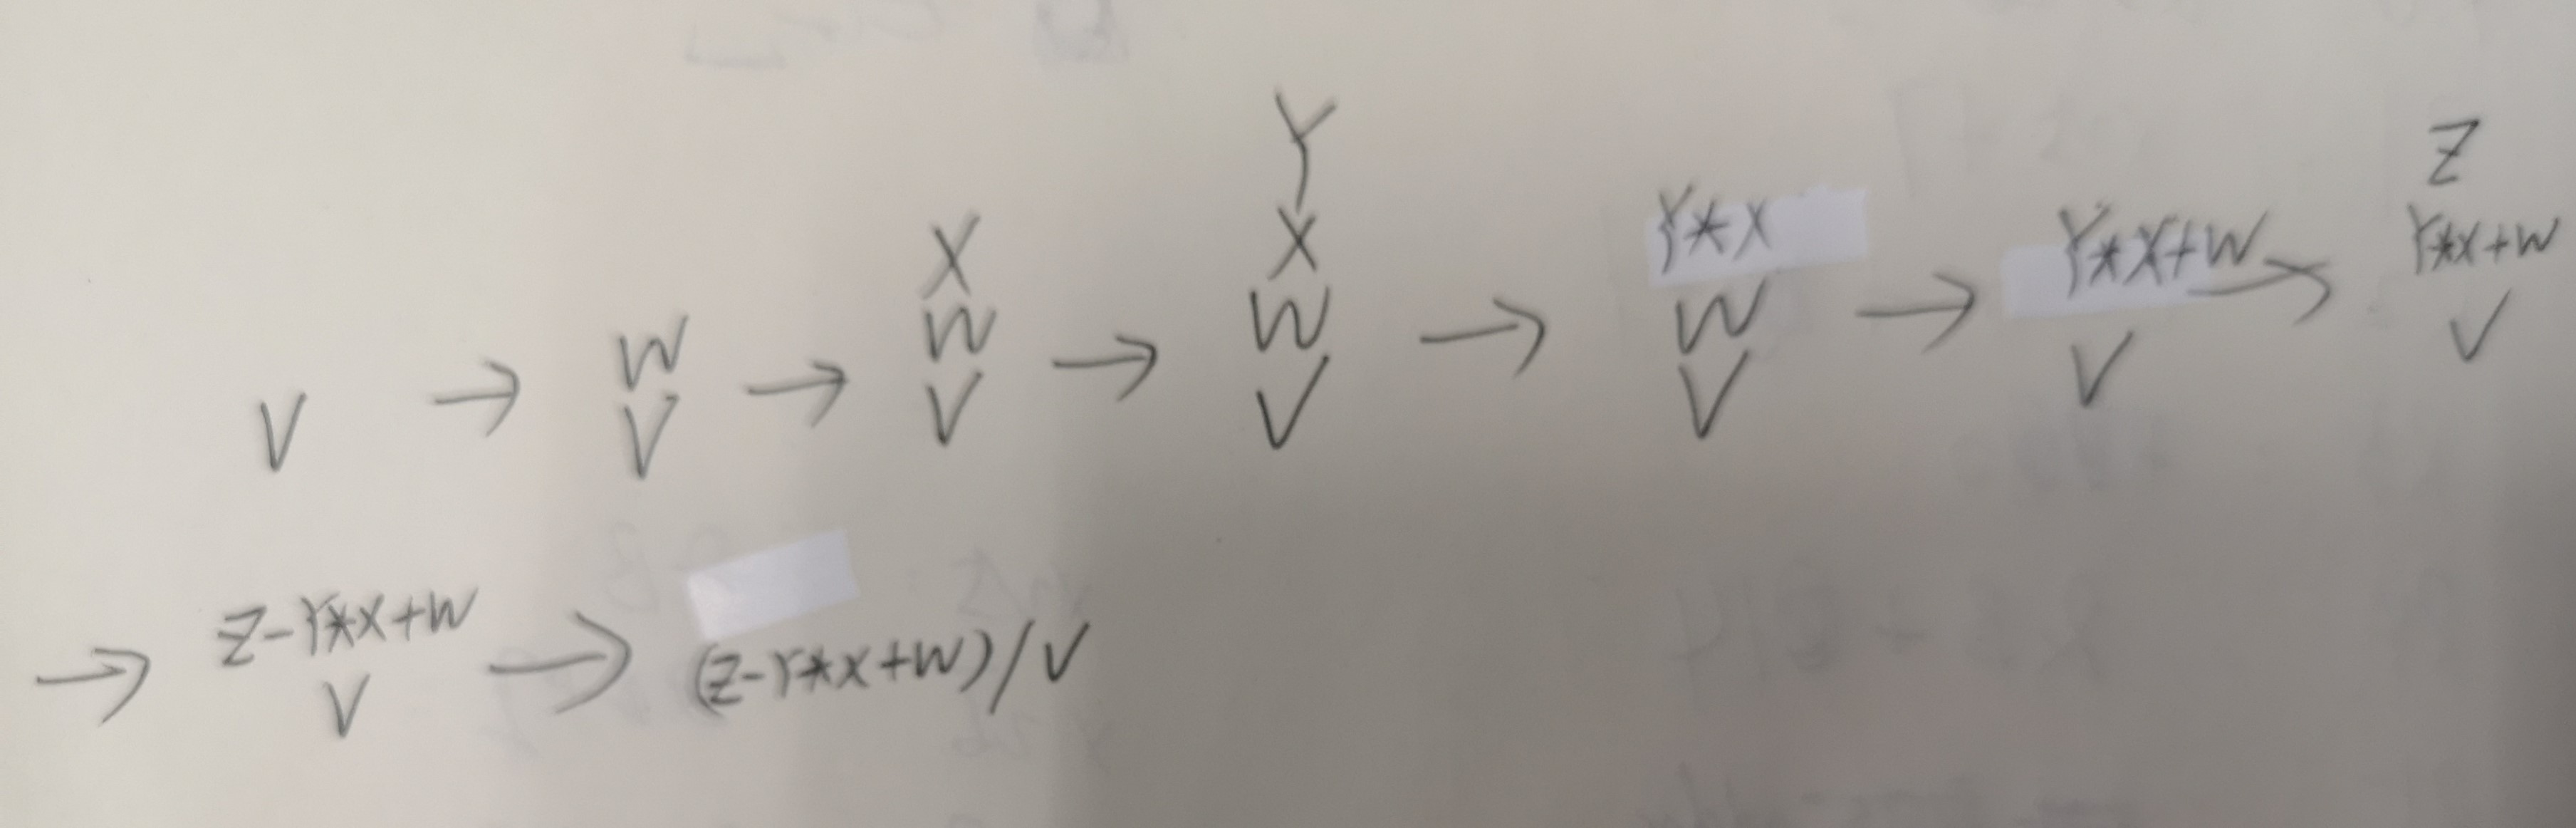
\includegraphics[scale=0.15]{6a.jpg}
		\label{6a}
	\end{figure}
	\subsection*{b}
	\begin{lstlisting}[language=C++]
	PUSH	C
	PUSH	A
	ADD
	PUSH	D
	PUSH	C
	PUSH	B
	SUB
	ADD
	PUSH	A
	MUL
	DIV
	\end{lstlisting}
	
	
		
\end{document}